\documentclass[compress]{beamer}
\usepackage{hyperref}
\usepackage{calligra}
\usepackage[T1]{fontenc}
\usefonttheme[onlymath]{serif}

\author{Zihang Wang}
\title{Phase Field Tutorial}
\subtitle{Introduction \& Mathematics 1}
\institute{Central South University}

\AtBeginSubsection[]
{
	\begin{frame}
		\tableofcontents[sectionstyle=show/shaded,subsectionstyle=show/shaded/hide,subsubsectionstyle=show/shaded/hide]
	\end{frame}
}

\usetheme{Berlin}

\setbeamertemplate{footline} {
    \begin{beamercolorbox}[ht=2.5ex,dp=1.125ex,
      leftskip=.3cm,rightskip=.3cm plus1fil]{title in head/foot}
      {\usebeamerfont{institute in head/foot}\usebeamercolor[fg]{institute in head/foot}\insertshortinstitute}
      \hfill
      {\centering\usebeamerfont{title in head/foot}\insertshortsubtitle}
      \hfill
      {\usebeamerfont{frame number}\usebeamercolor[fg]{frame number}\insertframenumber~/~\inserttotalframenumber}
    \end{beamercolorbox}
    \begin{beamercolorbox}[colsep=1.5pt]{lower separation line foot}
    \end{beamercolorbox}
}

\begin{document}

\begin{frame}
  \titlepage
  \begin{figure}[!h]
    \centering
    
\includegraphics[width=0.2\linewidth]{pic/csulogo.jpg}
    
\includegraphics[width=0.27\linewidth]{pic/MInDes_Icon.jpg}
  \end{figure}
\end{frame}

\begin{frame}
  \frametitle{Before Start\dots}
  \begin{itemize}
    \item Correct me if I'm wrong
    \item Stop me if you're confusing
    \item Questions welcome
    \item On/Off line Q\&A sessions are OK.
  \end{itemize}
\end{frame}


\begin{frame}
  \tableofcontents[currentsection, hideothersubsections, sectionstyle=show/show]
\end{frame}

\section{Introduction}
\subsection{{Phase Field Method}}

\begin{frame}
  \frametitle{What is Phase Field Method?}
  \begin{itemize}
    \item One of material simulation methods
    \item Use continuous variable describing interfaces
    \item Overcome the difficults of sharp interface
    \item Simulate phase evolution
  \end{itemize}
\end{frame}

\begin{frame}
  \frametitle{Phase Field and Field Variable}
  So, what is "Phase Field"?
  \begin{itemize}
    \item A variable (field variable / order parameter) across the simulation region
    \item The variable is depended temporally and spatially (Field)
    \item This variable can indicate a phase
    \item Conservative (finite variable sum across simulation field) or non-conservative (infinite variable sum across simulation field).
  \end{itemize}
\end{frame}

\subsection{Gonvering Equations}
\begin{frame}
  \frametitle{Two important equations}
  Two equations play really important roles in phase field method.

  \[
    \frac{\partial c_i}{\partial t} = \nabla \cdot M_{ij} \nabla \frac{\delta F}{\delta c_j \left( r,t \right)} \tag{Cahn-Hilliard}
  \]
  \[
    \frac{\partial \eta_p}{\partial t} = -L_{pq}\frac{\delta F}{\delta\eta_q\left( r,t \right)} \tag{Allen-Cahn}
  \]

  Here, \(c_i\) is concentration, \(t\) is time, \(\eta\) is order parameter, \(F\) is total free energy,
  \(M_{ij}\) and \(L_{pq}\) are some kind of mobilities.
  \begin{center}
    {\Huge How to solve these equations?}
  \end{center}
\end{frame}

\section{Mathematics}
\subsection{Taylor Formula}
\begin{frame}
  \frametitle{Where are these two equations from?}
  Where shall we start? We can observe these two equations.
  \bigbreak
  \(\nabla\) somehow stands for taking derivative spatially (to coordinates), while \(\frac{\partial}{\partial t}\)
  stands for taking derivative temporally (to time). These indicates that these derivatives are of great importance.
  \bigbreak
  Where are these equations from?


  To understand these two equations, one need dive into the origin of these two equations. We won't cover too much detail here,
  but will help you equiping with sufficient math tools to understand the derivations of these two equations.

  First we will introduce the \emph{Taylor Formula}.
\end{frame}

\begin{frame}
  \frametitle{Taylor Formula}
  Usually a free energy function/functional is complicated, especially when the second, third or higher order interfacial energies are considered.
  We wish that one can approximate a complicated function (\(f\)) with a polynomial (\(P\)) at one point (\(x_0\)) and in this point's neighbour.
  By saying approximate, we mean that:

  \begin{itemize}
    \item \(f(x_0) = P(x_0)\)
    \item \(f'(x_0) = P'(x_0)\), and this applies to higher derivatives until a order \(n\)
    \item \(\lim_{n\to\infty} f(x) - P(x) = \lim_{n\to\infty} r_n(x_0;x) = 0 \), where \(r_n\) is called \emph{remainder}
  \end{itemize}

\end{frame}

\begin{frame}
  \frametitle{Taylor Formula}
  So, to achieve this, we introduce \emph{Talor Formula}:
  \[
    f(x) = f(x_0) + \frac{f'(x_0)}{1!}\left( x-x_0 \right) + \dots + \frac{f^{(n)}(x_0)}{n!}\left( x-x_0 \right)^n
    +r_n( x_0;x )
  \]
  Here's an equivalent form:
  \[
    f(x+\delta{x}) = f(x) + \frac{f'(x)}{1!}\left( \delta{x} \right)+\dots+\frac{f^{n}(x)}{n!}\left( \delta{x} \right)^n+r_n(x;x+\delta{x})
  \]
  These formulas can help you eliminate the higher order terms as they are relatively small compared to the lower order terms. You shall see this
  formula been used widely. Please notice that here, `\(x\)' is a variable, but not specified to the `root' one. It could also depend on another variable,
  i.e., \(x(t)\).
\end{frame}

\subsection{Extrema with Constraint}
\begin{frame}
  \frametitle{How Energy Cooperates in Phase Field?}
  The most important part (or, possibly most complicate part) in these two evolution functions is the free energy `functional' (we shall
  introduce functional latter). The free energy functional here will define the system evolution direction, that is, to the energy minimal
  direction, according to the thermodynamical theory. Also, please notice that this minima comes with constraint that the concentration should
  be normalized to 1. So this question can be classified as `Extrema with Constraint'.
\end{frame}

\begin{frame}
  \frametitle{Lagrange Multiplier}
  To solve such question, a common way is using a method called `Lagrange Multiplier' method.

  Here's how to use it. Suppose we have a multi-variable function \(f : \mathbb{R}^n \supseteq U \to \mathbb{R}\), it's good enough that we could find
  a extrema under constraints \(\phi_j : U \to \mathbb{R}^m\) where \(m<n\).

  First, we construct a helper function
  \[F : \mathbb{R}^{n+1}\supseteq U' \to \mathbb{R},\]
  \[(x,\lambda) \mapsto f(x) - \sum_{i=1}^m \lambda_i \cdot \phi_i(x). \]
  So this helper function contains the original function and the constraint.
\end{frame}

\begin{frame}
  \frametitle{Lagrange Multiplier}
  Now take partial derivatives of helper function w.r.t. each variable, including \(\lambda\), then evaluate them to zero
  \[\frac{\partial F}{\partial x_i} = 0, 0\leq i \leq n;\]
  \[\frac{\partial F}{\partial\lambda_j} = 0, 0 \leq j \leq m.\]
  By now you will get a system of equations with \(n+m\) equations. Solving it and you will get the extrema of the function \(f\)
  under the constraints \(\phi_i\).
\end{frame}

\begin{frame}
  \frametitle{Why Lagrange Multiplier Works?}
  This is a little complicated. An illustrative explanation is that the extrema will appear
  at the point which the level set of \(f\) (that is, \(\left\{ x \in U \supseteq \Big| f(x) = f(x_0) = c \right\}\))
  tangents with constraints surfaces/curves (these constraints usually appears as \(\phi_i(x) = 0\)). That is, the gradient
  of \(f\) must be orthogonal to the tangent vector of constraints surfaces/curves.

  \begin{figure}[!h]
    \centering
    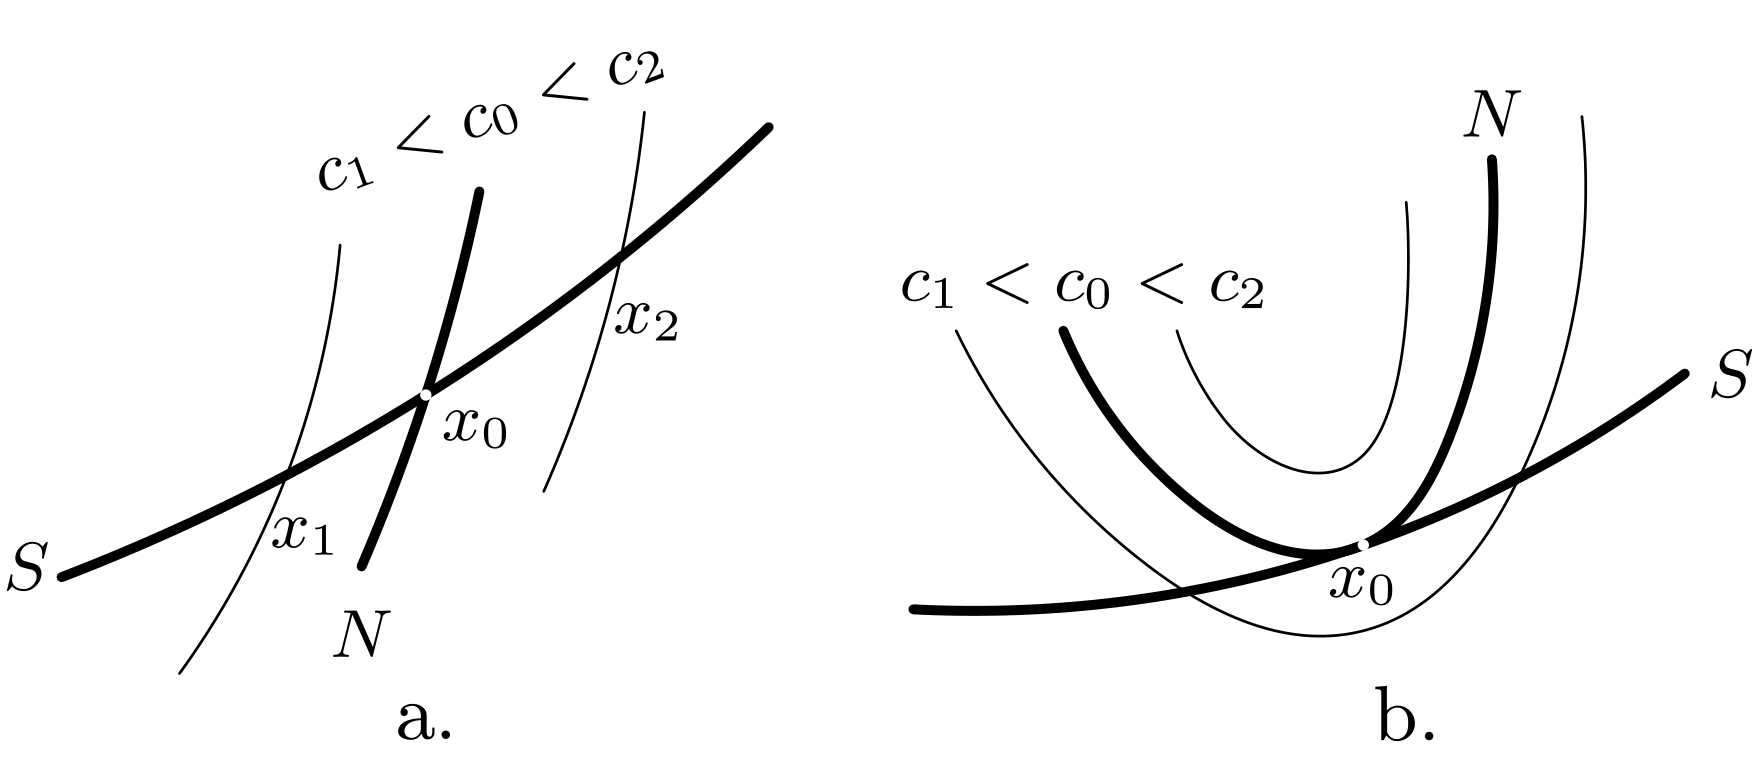
\includegraphics[width=0.7\linewidth]{pic/Lagrange.png}
  \end{figure}

\end{frame}

\subsection{Variational Derivative}
\begin{frame}
  \frametitle{So What is Functional? Set Map?}
  We mentioned `Free Energy Functional' But what's that?
  Here we start from the most basic `function', i.e., \emph{map}.
  \begin{block}{Set Map (Mapping)}
    A \emph{map} (or, \emph{mapping}) \(\phi\) is a set of arrows from elements in one set \(\mathbf{S}\) to elements in another set \(\mathbf{T}\).
    \(\mathbf{S}\) is called \emph{domain}, and \(\mathbf{T}\) is called \emph{codomain}.
    A map satisfies that each elements in \(\mathbf{S}\) has a unique arrow to only one element \(\mathbf{T}\). We say \(\phi\) maps \(\mathbf{S}\) to \(\mathbf{T}\),
    and denotes \(\phi : \mathbf{S} \to \mathbf{T}\). Suppose \(x \in \mathbf{S}\), we use notation \(x \mapsto \phi(x)\) to define map explicitly.
  \end{block}
  So you can see, here we define the `map' as something like `function' that one might be familiar with already. While, How to define \emph{function}?
\end{frame}

\begin{frame}
  \frametitle{Function and Functional}
  \begin{block}{Function}
    A \emph{function} is a map that its codomain is a \emph{number field} (for example, \(\mathbb{R}, \mathbb{C}\)).
  \end{block}
  As a math object, functions can be grouped into a set. Replace the domain of function (subset of number field) with
  set of functions, then you get:
  \begin{block}{Functional}
    A (classical) functional is a map that its domain is set of functions, and its codomain is a number field.
  \end{block}
  Now it should be clear that, functional is nothing but a special map, output a number when inputing a function.
\end{frame}

\begin{frame}
  \frametitle{A long foot note}
  \begin{enumerate}
    \item Mapping, function have different meaning depending on the context. Some authors prefer using map, mapping, function interchangeably as
          arrows from set to set, while some authors, especially in algebraic studying, like Serge Lang, prefer seperate functions from mappings.
    \item Modern mathematical definition of fuctional is mappings from vector space to its base field,
          or a synonymous of linear form, while to study the variational calculus, `functional' mentioned here is `in classical meaning', i.e. `function of function',
          and  usually in form \[J\left[ y \right]=\int_{x_1}^{x_2}L(x,y(x),y'(x)) \,\mathrm{d}x.\]
          Check \href{https://en.wikipedia.org/wiki/Functional_(mathematics)}{\color{blue}Wiki} for more information.
  \end{enumerate}
\end{frame}

\begin{frame}
  \frametitle{Brachistochrone curve}
  Great, now we know what's functional. But what is its derivative? Let's start from variations.

  Variations are raised from brachistochrone curve problem, saying that which curve between two fixed points A and B is
  the fastest path for frictionlessly movement under gravitational field. To solve this problem, variations and variational calculus are needed.
  \begin{figure}
    \centering
    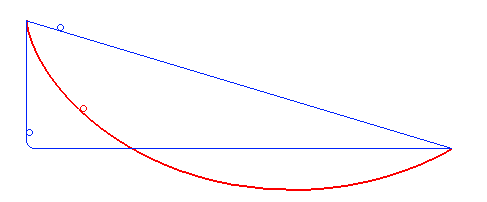
\includegraphics[width=0.7\linewidth]{pic/Brachistochrone.png}
  \end{figure}
\end{frame}

\begin{frame}
  \frametitle{Variations and Functional Deriavtive}
  To start with, consider that a function is already the fastest path, then any other path will not be the fastest path (in a region). If one introduces a small
  variation to the path (that's where `variation' comes), then the varied path will take longer time. If one can process this variation as somehow like differential,
  then just let the `derivative of path to path variation' be evaluated to zero, the path solved will be the fastest path.
  \bigbreak
  Here, `variation' is the small difference between two functions with the same domain,
  `derivative of path to path variation' is the functional derivative.
  \bigbreak
  But how to calculate the functional derivative, then evaluate it to zero and get the fastest path, or, extrema function?
\end{frame}

\begin{frame}
  \frametitle{Euler-Lagrange Equation}
  Fortunately, here is a well-known method called \emph{Euler-Lagrange Equation} (abbreviation `E-L equation') that can help one to determine the extrema and give the functional derivative.
  Here it is:
  \bigbreak
  Consider a funcional: \[J\left[ y \right] = \int_{x_1}^{x_2} L(x,y(x),y'(x))\,\mathrm{d}x\].
  Then, the Euler-Lagrange Equation of this functional is:
  \[\frac{\partial L}{\partial f} - \frac{\mathrm{d}}{\mathrm{d} x}\frac{\partial L}{\partial f'}=0,\]
  where \(f\) is the extremal, and the left part of this equation is so called `Functional Derivative.'
\end{frame}

\begin{frame}
  \frametitle{For braver}
  If you are interested in derivation of E-L equation, here it is.
  \bigbreak
  Consider a function \(\eta(x)\) that takes \(0\) at end points \(x_1\),\(x_2\) of variable \(x\). Multiply this with a small number \(\varepsilon\),
  we get a variation \(\delta f = \varepsilon\eta\). Suppose the extrema (suppose minimum, the same as maximum)
  \(f\) of functional \(L(x,y,y')\). Then we get:
  \(J\left[ f \right] < J\left[ f+\delta f \right] = J\left[ f+\varepsilon\eta \right]\).
  Now fix this arbitrary function \(\eta\), define a function \(\Phi\left( \varepsilon \right) = J\left[ f+\varepsilon\eta \right].\)
  As \(f\) is the minimum function, then
  \[\Phi'\left( 0 \right) = \int_{x_1}^{x_2} \frac{\mathrm{d} L}{\mathrm{d} \varepsilon}\Big|_{\varepsilon} = 0 \,\mathrm{d}x = 0.\]

\end{frame}

\begin{frame}
  \frametitle{For braver}
  Then, consider \(L(x,y,y')\) as nothing but a normal two variables function, i.e. \(L(y(\varepsilon),y'(\varepsilon))\), where \(y = f+\varepsilon\eta\) and \(y' = f'+\varepsilon\eta'\), then taking its derivative:
  \[\frac{\mathrm{d} L}{\mathrm{d} \varepsilon} = \frac{\partial L}{\partial y}\frac{\mathrm{d} y}{\mathrm{d} \varepsilon}+\frac{\partial L}{\partial y'}\frac{\mathrm{d} y'}{\mathrm{d} \varepsilon}.\]
  \[\frac{\mathrm{d} L}{\mathrm{d} \varepsilon} = \frac{\partial L}{\partial y}\eta+\frac{\partial L}{\partial y'}\eta'.\]
  Therefore, taking this back to \(\Phi'(0)\) and integrate by part:
  \[\Phi'\left( 0 \right) = \int_{x_1}^{x_2} \frac{\partial L}{\partial f}\eta+\frac{\partial L}{\partial f'}\eta'\,\mathrm{d}x =
    \int_{x_1}^{x_2} \left( \frac{\partial L}{\partial f}-\frac{\mathrm{d} }{\mathrm{d} x}\frac{\partial L}{\partial f'} \right)\eta\,\mathrm{d}x+\frac{\partial L}{\partial f'}\eta\Big|_{x_1}^{x_2}\]
\end{frame}

\begin{frame}
  \frametitle{For braver}
  By our definition of \(\eta\), the last term \(\frac{\partial L}{\partial f'}\eta\Big|_{x_1}^{x_2}\) will be zero. Then free \(\eta\) as a arbitrary function, to make \(\Phi'(0) = 0\),
  the integrated inner part should be \(0\)
  \[\frac{\partial L}{\partial f}-\frac{\mathrm{d} }{\mathrm{d} x}\frac{\partial L}{\partial f'} = 0.\]
  And the variational derivative should be:
  \[
    \frac{\delta J[y]}{\delta y} = \frac{\partial L}{\partial y}-\frac{\mathrm{d} }{\mathrm{d} x}\frac{\partial L}{\partial y'}
  \]
  That's it, you derivated E-L equation by yourself. But in a relaxed way. There are many good resources about variational calculus and
  functional, asking for a bunch of time and effort to master them. Please search them if you like.
\end{frame}


\subsection{Vector Calculus}
\begin{frame}
  \frametitle{Finally, \(\nabla\)}
  After some preparation, we finally got everything to understand Cahn-Hilliard and Allen-Cahn equations, except for the
  notation \(\nabla\). What's that? We assume you have alreday know the `partial derivative', and suppose there is a function \(f\)
  of coordinates \(x_1,x_2,x_3\). Then:
  \[\nabla = \hat{x}_1 \frac{\partial }{\partial x_1} + \hat{x}_2\frac{\partial }{\partial x_2}+\hat{x}_3\frac{\partial }{\partial x_3},\]
  where \(\hat{x}_i\) mean the base vectors. If we adopt for the matrix form, then:
  \[
    \nabla =
    \begin{bmatrix}
      \frac{\partial }{\partial x_1} \\
      \frac{\partial }{\partial x_2} \\
      \frac{\partial }{\partial x_3}
    \end{bmatrix}
  \]
\end{frame}

\begin{frame}
  \frametitle{Del Operator}
  Things are getting clearer. This notation, \(\nabla\), is a \emph{operator} called `del'. An operator takes function to another function, and this
  operator is more special, it is linear and can be written as a vector. You can image how this operator cooperates with functions in various way. Here
  we write them explicitly:

  Acting directly on a scalar (Gradient):
  \[\nabla f = \hat{x}_1 \frac{\partial f}{\partial x_1} + \hat{x}_2\frac{\partial f}{\partial x_2}+\hat{x}_3\frac{\partial f}{\partial x_3}\]
  Dot product with a vector (Divergence):
  \[\nabla \cdot \hat{f} = \frac{\partial f_1}{\partial x_1} + \frac{\partial f_2}{\partial x_2}+\frac{\partial f_3}{\partial x_3}\]
\end{frame}

\begin{frame}
  \frametitle{Del Operator}
  Cross product with a vector (Curl):
  \[\nabla \times \hat{f} = \begin{vmatrix}
      \hat{x}_1                      & \hat{x}_2                      & \hat{x}_3                      \\
      \frac{\partial }{\partial x_1} & \frac{\partial }{\partial x_2} & \frac{\partial }{\partial x_3} \\
      f_1                            & f_2                            & f_3
    \end{vmatrix}
  \]
  \[ = \hat{x}_1\left( \frac{\partial f_3}{\partial x_2}-\frac{\partial f_2}{\partial f_3} \right)
    + \hat{x}_2\left( \frac{\partial f_1}{\partial x_3}-\frac{\partial f_3}{\partial f_1} \right)
    + \hat{x}_3\left( \frac{\partial f_2}{\partial x_1}-\frac{\partial f_1}{\partial x_2} \right)
  \]
  What we will encounter mainly is the first case, gradient, taking a function and give a vector valued function.
  And please notice that here, gradient can be considered as `derivative w.r.t. coordinates'.
\end{frame}
\begin{frame}
  \frametitle{Del with functions}
  What if \(\nabla\) is acted on composed function? what if the composed function is a scalar function times vector function?
  Please try it yourself!
  \begin{block}{Q1}
    Suppose there are three functions:\(\phi,\psi : \mathbb{R}^3 \to \mathbb{R}\) and \(\hat{f} : \mathbb{R} \to \mathbb{R}^3\).
    Please prove:
    \[\nabla\left( \phi\psi \right) = \phi\nabla\psi + \psi\nabla\phi\]
    \[\nabla\cdot\left( \phi\hat{f} \right) = \nabla\phi\cdot\hat{f} + \phi\nabla\cdot\hat{f}\]
    By proving these, you should what we meant by `derivative w.r.t. coordinates'.
    \bigbreak
    \emph{Hint: prove them by the definition of \(\nabla\)}
  \end{block}
\end{frame}


\section{Summary}
\subsection{Two equations, and more}
\begin{frame}
  \frametitle{Combine What We Got}
  By now we got many math tools to understand the two equations used in phase field simulation. Let's review
  these two equations:
  \[
    \frac{\partial c_i}{\partial t} = \nabla \cdot M_{ij} \nabla \frac{\delta F}{\delta c_j \left( r,t \right)} \tag{C-H}
  \]
  \[
    \frac{\partial \eta_p}{\partial t} = -L_{pq}\frac{\delta F}{\delta\eta_q\left( r,t \right)} \tag{A-C}
  \]
  so, we can say that, the C-H equation means that, the concentration evolution rate is proportional to the divergence
  of the chemical potential flux. That is something like Fick's second law in diffusion (indeed there is relationship).
  And the A-C equation indicates that the order parameter evolution rate is proportional to its potential.
\end{frame}

\begin{frame}
  \frametitle{Different Variable for Different Equation}
  Which equation should be used to evolute the system? Maybe you can get some clues from the equations themselve, by considering
  when the system is balanced. Divergence here indicates that C-H equation is for \emph{conservative variable}, for example,
  concentration, phase fraction, as the sum of these variable should be a finite value. While A-C equation is for \emph{non-conservative
    variable}, such as order parameter. You shall see these two equations in the tutorial 4 and 5 in the near future.
\end{frame}

\begin{frame}
  \frametitle{Free energy functional form}
  With the mathematical tools at hand, you can derivate the explicit form of the gonvering equations by yourself if
  the free energy functional is given. But wait, what's the general form of these functional?
  \bigbreak
  The functional we encounter usually has form of:
  \[F(x,c,\nabla c) = \int_{\Omega} f(c,\eta) + \kappa_c
    \left( \nabla{c} \right)^2 +\kappa_\eta\left( \nabla{\eta} \right)^2 + S\,\mathrm{d}v,\]
  where \(f(c,\eta)\) is the chemical energy function (sometimes called bulk energy), and the second and third term usually
  refered as \emph{interfacial energy}, and \(S\) stands for other free energy contribution.
\end{frame}

\begin{frame}
  \frametitle{Try it!}
  Although we won't cover too much on the physical meaning of this functional, you can still try to subsitute this example
  free energy functional into the equations (treat mobility \(M_{ij}\) as constant).
  \bigbreak
  \begin{block}{Q2.}
    Please try to subsitute the following free energy functional into C-H equation get the gonvering equation:
    \[F\left( x,c,\nabla c \right) = \int_{\Omega} f(c) + \frac{\kappa}{2}\left( \nabla c \right)^2 \,\mathrm{d}v.\]
    \bigbreak
    \emph{Hint: E-L equation, and `\(\nabla\)' is nothing but derivative.}
  \end{block}
\end{frame}

\begin{frame}
  \frametitle{Resources}
  Here are some resources that can help you with today's topic.
  \begin{itemize}
    \item \href{https://www.bilibili.com/video/BV1oC4y147CU/}{\color{blue}Bilibili video} about Phase field modelling. I recommend part 60-64, related to variational
          calculus. This video series helps me a lot.
    \item Vector calculus: \emph{Introduction to Electrodynamics} by David J. Griffiths, and some books about \emph{Methods for Mathematical Physics}. They all have good
          introduction to the vector calculus, especially focusing on the usage of calculation rules.
    \item Functional derivatives (Variational Calculus): Again, please refer to some physics textbooks. You may find many resources in mathematical context,
          that may not be suitable for calculation. I personally recommend
          \href{https://en.wikipedia.org/wiki/Functional_derivative}{\color{blue}Wikipedia},
          \href{https://physicspages.com/pdf/Field\%20theory/Functional\%20derivatives\%20-\%20more\%20examples.pdf}{\color{blue}a samll note},
          \href{https://www.jiaxuanli.me/Homepage/doc/Mathematical_Method/chpp20.pdf}{\color{blue}another note}, and again, some physical books.
  \end{itemize}
\end{frame}

\begin{frame}
  \begin{center}
    {\Huge \calligra Thanks!}
    \bigbreak
    {\huge Any questions are welcomed!}
  \end{center}
\end{frame}

\end{document}
